\subsection{Gateway}
	Un \textit{gateway} è una componente localizzata all'interno di un'azienda e permette di rendere uniforme l'interfaccia di accesso ai dati dei dispositivi configurati all'interno del gateway stesso.
	Dei gateway è possibile inoltre configurare funzioni di accumulo dei pacchetti contenenti i dati dei sensori o di impostare alcuni timer al termine dei quali effettuare l'invio dei dati all'interno dei rispettivi topic di Kafka tramite un producer;
	Tutte le configurazioni vengono ricevute da topic di Kafka adibiti esclusivamente a questa funzione.
	
	\subsubsection{Diagramma dei package}%%%%%%%%%%%%OK
	  	\begin{figure}[H]
			\centering
			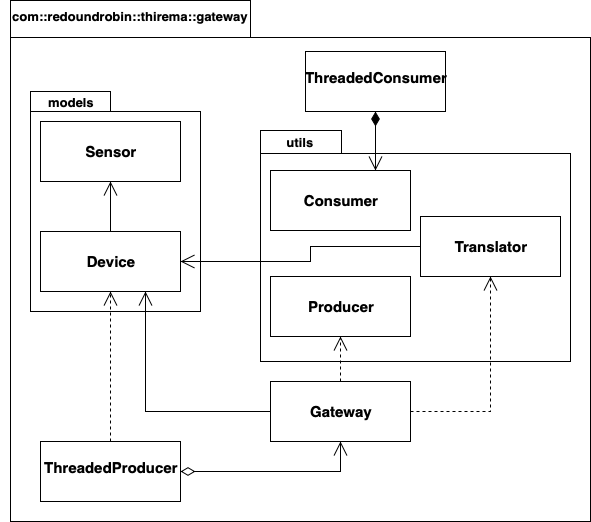
\includegraphics[scale=0.550]{res/images/GATEWAY/GatewayPackage.png}
			\caption{Diagramma delle classi per la componente gateway}
		\end{figure}		

		\begin{landscape}
	\subsubsection{Diagramma delle classi}%%%%%%%%%%%%%%%%%%%%%%%OK
	  	\begin{figure}[H]
			\centering
			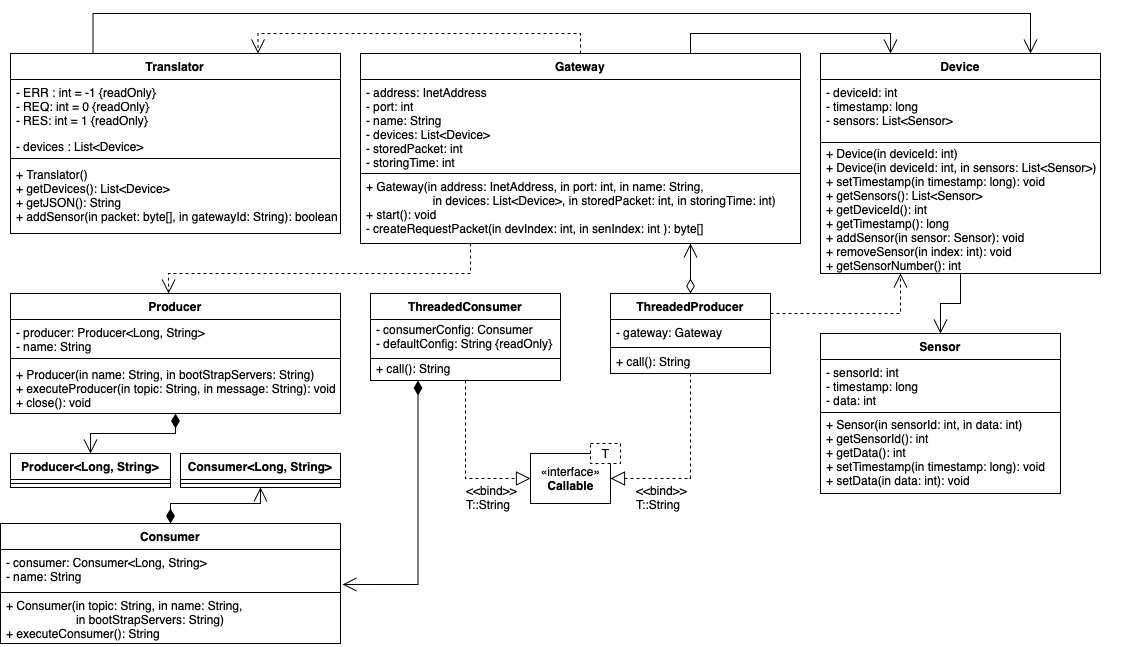
\includegraphics[scale=0.500]{res/images/GATEWAY/ClassiGateway.png}
			\caption{Diagramma delle classi per la componente gateway}
		\end{figure}	
		\end{landscape}
		\begin{landscape}
	\subsubsection{Diagramma di sequenza}
	  	\begin{figure}[H]
			\centering
			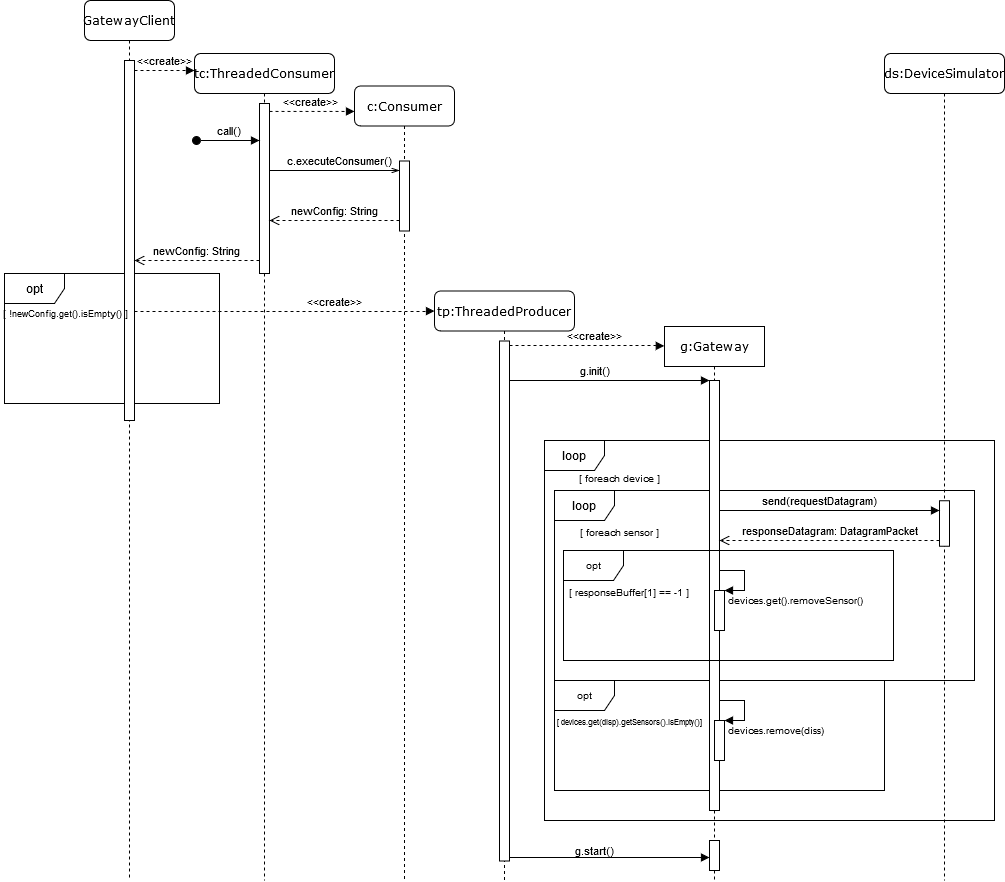
\includegraphics[scale=0.500]{res/images/GATEWAY/RichiestaInvioGateway.png}
			\caption{Diagramma di sequenza che rappresenta la richiesta di un dato e il conseguente invio del messaggio a un topic di Kafka}
		\end{figure}
		
		Nel diagramma precedente sono stati mezionati in minima parte sia il simulatore dispositivi per una questione di continuità che il consumer per mostrare nella sua interezza ciò che avviene all'interno del gateway.
		\end{landscape}
	\subsubsection{Diagramma di attività}
		\begin{figure}[H]
			\centering
			\includegraphics[scale=0.500]{res/images/GATEWAY/gateway.start().png}
			\caption{Diagramma di attività che rappresenta un'iterazione all'interno del metodo start() della classe Gateway}
		\end{figure}








